10. \begin{figure}[ht!]
\center{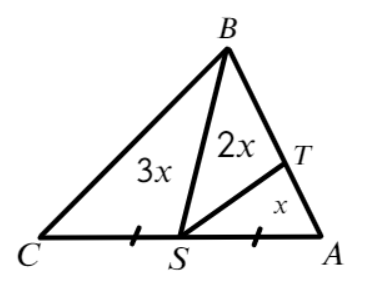
\includegraphics[scale=0.35]{g9-10.png}}
\end{figure}\\
Если треугольники имеют общую высоту, их площади относятся так же, как основания, к которым проведена эта высота. Поэтому $S_{\Delta ATS}=x,\ S_{\Delta BTS}=2x,$ а $S_{\Delta BCS}=S_{\Delta BAS}=x+2x=3x.$ Поэтому $\cfrac{S_{\Delta ATS}}{S_{CBTS}}=\cfrac{x}{3x+2x}=\cfrac{1}{5}.$\\
